% arara: pdflatex
% arara: biber
% arara: makeindex
% arara: nomencl
% arara: pdflatex
% arara: pdflatex

\documentclass[a4paper,12pt]{article}
%\RequirePackage[l2tabu,orthodox]{nag}

\usepackage{upreport}
\addbibresource{report.bib}
\title{Sample report}
\author{Carl Sandrock}
\studentnumber{1234567}
\subject{CXX XXX}
\date{\today}

%Nomenclature unit command
\newcommand{\nomunit}[1]{%
\renewcommand{\nomentryend}{\hspace*{\fill}#1}}

% Create a custom user command or run the following 
%  makeindex %.nlo -s nomencl.ist -o %.nls
% execute this command after compiling your file once, then compile a second time to generate a nomenclature table

\begin{document}
\maketitle
\makecoverpage

\pagestyle{plain}
\thispagestyle{plain}
\pagenumbering{roman}

\begin{center}
\LARGE\textbf{\thetitle}
\end{center}

\section*{Abstract}
\addcontentsline{toc}{section}{Abstract}%
This sample report contains information in the main text, visible when the report is compiled as well as in comments in the .tex file. Please note both.

Make sure you have the latest version of this repository by using Git to clone the repository or by downloading from \url{https://github.com/ChemEngUP/ce-up-latex-templates/}.
\setcounter{page}{3}

\newpage
\tableofcontents

\iftotalfigures%
\newpage%
\listoffigures%
\fi

\iftotaltables%
\newpage%
\listoftables%
\fi

\newpage

%\chapter*{Nomenclature}
\printnomenclature
\newpage

\pagestyle{plain}
\setcounter{page}{1}
\pagenumbering{arabic}

% Note: To edit the abstract, edit the file abstract.tex

\section{Introduction} 
Background, problem statement, purpose, method, scope.

\section{Theory}
Summary of the relevant theory, including ample references. You can refer to citations like~\textcite{bruckmanmandersloot} for an inline reference or \parencite{bruckmanmandersloot} to get the citation in parentheses. You can also cite multiple authors~\parencite{mandersloot,bruckmanmandersloot}. For examples on graphics see \ref{sec:Results}.

The height $h$ \nomenclature{h}{Height \nomunit{m}} was measured as a function of time $t$ \nomenclature{t}{time \nomunit{s}}.  The relationship between $h$ and $t$ was found to be 
\begin{equation}
  \label{eq:commaexample}
  h(t) = h_0 - \lambda t
\end{equation}
where $h_0$ is the initial height and $\lambda$ is an experimentally
determined constant.  It was also determined that the velocity
$\mathbf{v}$ was a function of the position $\mathbf{x}$ given by
$f(\mathbf{v}) = \beta \mathbf{x} + \sin(\alpha)$ and that in general
$h_{\mathrm{max}} \leq 5$ m.

Dynamic analysis showed that the system could be represented by
Equation~\ref{eq:matexample}
\begin{equation}
  \label{eq:matexample}
  G(s) = \frac{1}{s+1}\left [ 
    \begin{array}{cc} 
      3 & \log{b} \\ 
      2 & \num{1.1} 
    \end{array} \right ]
\end{equation}

Therefore, the model was revised to
\begin{equation}
  \frac{\partial f}{\partial t} = 5t + g(t) \qquad \frac{\mathrm{d} g}{\mathrm{d} t} = t + f(t) \qquad A = \int_a^b f(t) \mathrm{d} t
\end{equation}

For chemical symbols, use the mhchem package to get nicely typeset chemical
names. You can use it in the text like \ce{H2O} or in equations like below:
\begin{align}
  \label{eq:chemexample}
  \ce{H2 + O2 &-> H2O} \\
  \ce{H2O + H+ &-> H3O+}
\end{align}

\section{Experimental}
\subsection{Materials}

\subsection{Apparatus}

\subsection{Analytical instruments}

\subsection{Planning}

\subsection{Methods}

\section{Results and discussion}
\label{sec:Results}
Supporting evidence, most important results first. Use graphs and tables where possible. Explain the observed correlations between variables.

\subsection{Tables}
Prefer simple tables like Table~\ref{tab:simpletabexample}.
\begin{table}[htbp]
  \centering
  \caption{Example of a simple table}
  \label{tab:simpletabexample}
  \begin{tabular}{llS}
    \toprule
    Head 1 & Head 2 & {Head 3} \\
    \midrule
    Item 1 & value 1 & 12.3 \\
    Item 2 & value 1 & 1.2 \\
    Item 3 & value 1 & 4.5 \\
    Item 4 & value 1 & 0.053 \\
    \bottomrule
  \end{tabular}
\end{table}
In some cases you may want to use a
more complicated table like Table~\ref{tab:tabexample}. Notice that the decimals
of the right hand column are aligned using the \texttt{S} column type which
comes from the siunitx package.

\begin{table}[htbp]
  \centering
  \caption[Short caption for table of tables]{Example of a complicated table (adapted from \textcite{fear})}
  \label{tab:tabexample}
  % This minipage is only necessary when you need footnotes. For most tables you
  % can use the simple format.
  \begin{minipage}{0.5\textwidth}
    \begin{centering}
      \begin{tabular}{@{}llS@{}} \toprule 
        \multicolumn{2}{c}{Item}                                               \\ 
        \cmidrule(r){1-2} 
        Animal                    & Description & {Price\textsuperscript{a} (R)} \\ 
        \midrule 
        Gnat                      & per gram    & 13.65                  \\ 
                                  & each        & 0.01                   \\ 
        Parrot\textsuperscript{b} & stuffed     & 92.50                  \\ 
        Emu                       & stuffed     & 33.33                  \\ 
        Armadillo                 & frozen      & 8.99                   \\ 
        \bottomrule 
      \end{tabular}                                                            \\
    \end{centering} 
    \vspace{1em}
    \textsuperscript{a} As of 2004                                             \\
    \textsuperscript{b} Norwegian blue only
  \end{minipage}
\end{table}

Note that the \verb|\footnote| command doesn't work as one would like in
tables. The source for this table includes a workaround.

\subsection{Figures}
The simplest form of a figure is shown in Figure~\ref{fig:samplefigure}.

\begin{figure}[htbp]
  \centering
  % notice we specified the size of the figure in the Python file
  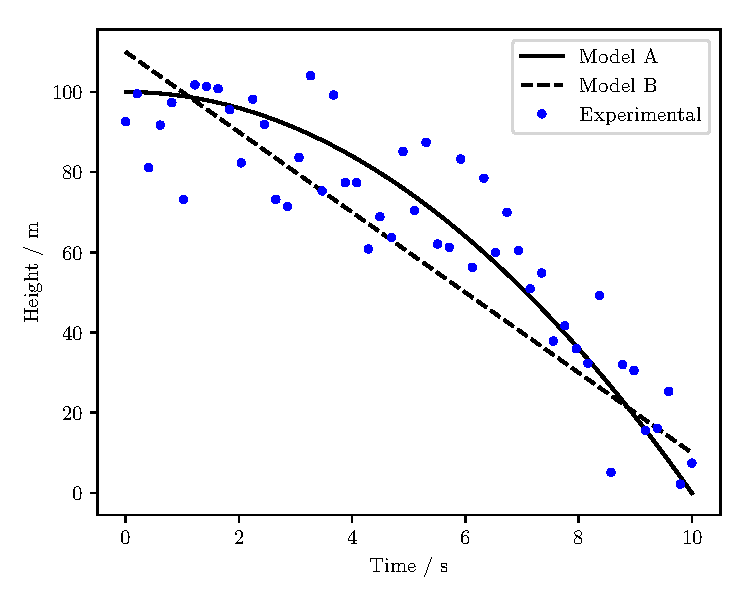
\includegraphics{Figures/samplefigure.pdf}
  \caption[Short caption which will be in the table of figures]{Example of a figure.  Note that the line types are easy to
    distinguish without a colour display.  Include a citation in the caption if the figure is from referred source. To update this figure, run samplefigure.py and recompile the document.}
  \label{fig:samplefigure}
\end{figure}

An important thing to understand about graphics in \LaTeX\ is that it does
not respect font size or line size specifications from the included graphics.
Instead it sees an image as single unit which is all scaled together. You can
see the difference between scaling a figure down inside \LaTeX\ and using a
custom-build scaled down version in figure~\ref{fig:scalingexample}

\begin{figure}[htbp]
  \centering
  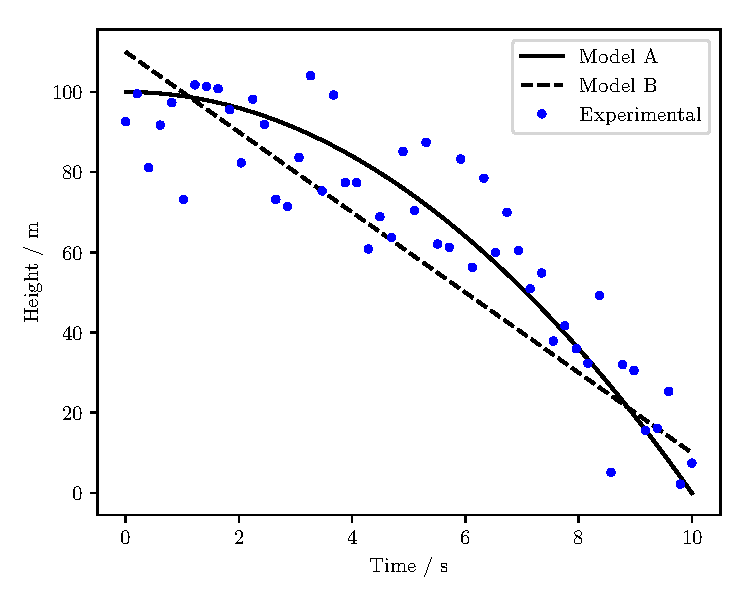
\includegraphics[width=3in]{Figures/samplefigure.pdf}
  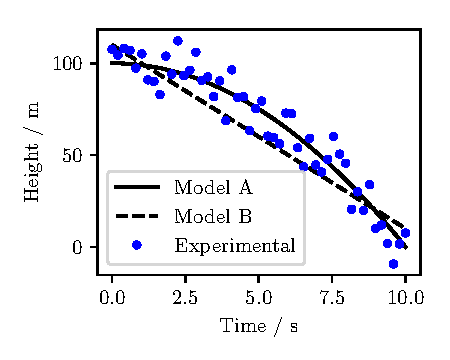
\includegraphics{Figures/samplefigure_halfsize.pdf}
  \caption{Two graphics side by side. The one on the left is the same as
    in Figure~\ref{fig:samplefigure}. Notice that the fonts are too small,
    the lines are too thin, and the dots are too small.}
  \label{fig:scalingexample}
\end{figure}

A common misunderstanding of this effect is that the font size is too small.
Editors unfamiliar with \LaTeX\ will often simply ask for the font size to be
bigger, but this does not address the other elements like the size of the lines,
the size of dots and so on. To obtain regular results, the safest option is to
specify the figure size in the software you are using to produce the figures.
The samplefigure.py file included with this template shows how these figures
were generated. Notice that the font size was not specified.

If you have multiple figures that need to be grouped together, it is useful to
make use of subfigures as shown in Figure~\ref{fig:subcaptionfigure}. Each
subfigure can be referenced as Figure~\ref{fig:1b}.


\begin{figure}[htbp]
	\begin{subfigure}[b]{0.5\textwidth}
		\centering
    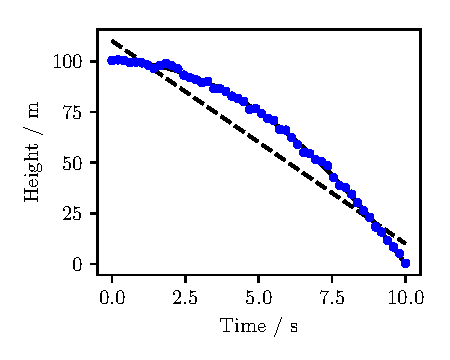
\includegraphics{Figures/noise_001_model.pdf}
		\caption{Noise factor = \num{1}}\label{fig:1a}
	\end{subfigure}\hfill  
	\begin{subfigure}[b]{0.5\textwidth}
		\centering
    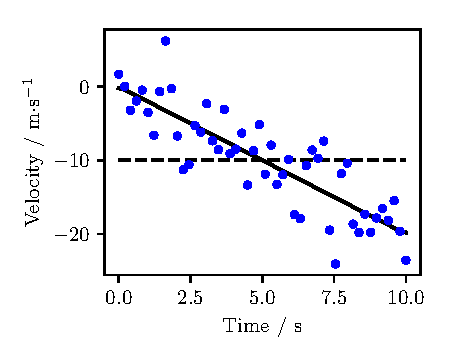
\includegraphics{Figures/noise_001_derivative.pdf}
		\caption{Noise factor = \num{1}}\label{fig:1b}
	\end{subfigure}\hfill
	\begin{subfigure}[b]{0.5\textwidth}
		\centering
    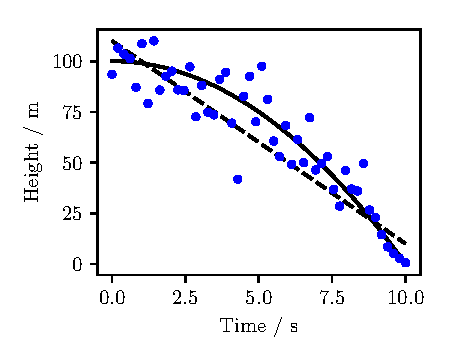
\includegraphics{Figures/noise_010_model.pdf}
		\caption{Noise factor = \num{10}}\label{fig:1c}
	\end{subfigure}\hfill
	\begin{subfigure}[b]{0.5\textwidth}
		\centering
    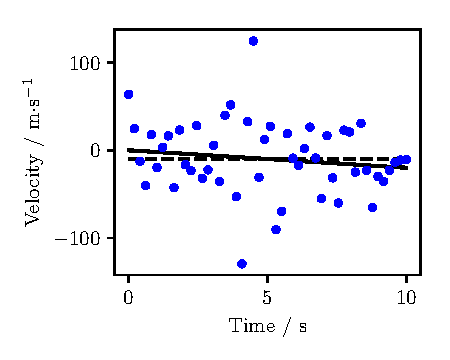
\includegraphics{Figures/noise_010_derivative.pdf}
		\caption{Noise factor = \num{10}}\label{fig:1d}
	\end{subfigure}\hfill
	\begin{subfigure}[b]{0.5\textwidth}
		\centering
    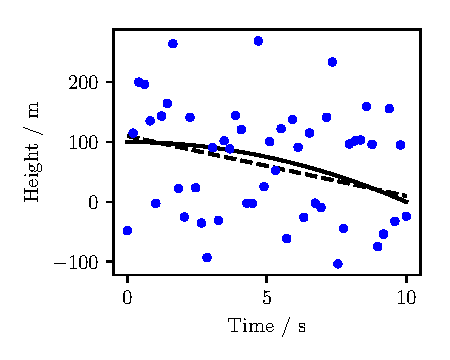
\includegraphics{Figures/noise_100_model.pdf}
		\caption{Noise factor = \num{100}}\label{fig:1e}
	\end{subfigure}\hfill
	\begin{subfigure}[b]{0.5\textwidth}
		\centering
    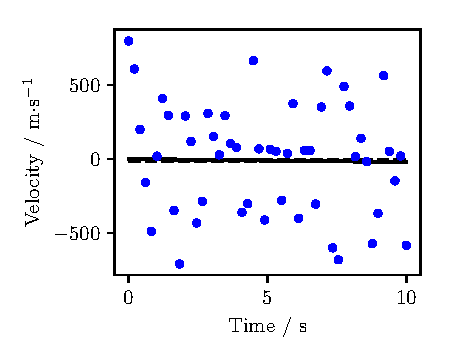
\includegraphics{Figures/noise_100_derivative.pdf}
		\caption{Noise factor = \num{100}}\label{fig:1f}
	\end{subfigure}
	\caption[Short caption which will be in the table of figures]{Example of a figure that contains multiple subfigures.  To update this figure, run samplefigure.py and recompile the document.}
	\label{fig:subcaptionfigure}
\end{figure}

For more options on using subfigures and more complicated subcaptions, see the package documentation at \url{https://gitlab.com/axelsommerfeldt/caption} 

\subsection{Numbers and units}
Numbers are shown with a decimal point, spaces between thousands and $\times 10^x$ notation rather than computer notation (\num{12345.12345e-12}).

SI units should be favoured except where conversion would be
uncomfortable (refer to a \SI{20}{psi} pressure limit rather than
\SI{137.895}{\kilo\pascal}).

Use standard SI prefixes instead of scientific notation unless a large variation in
numbers occurs (use \SI{1}{\nano\meter} instead of \SI{1e-9}{\meter}).

\section{Conclusions and recommendations}
Main findings.
No new information.

\printbibliography
\appendix
\renewcommand{\thefigure}{\thesection.\arabic{figure}}
\renewcommand{\thetable}{\thesection.\arabic{table}}
\renewcommand{\thepage}{\thesection.\arabic{page}}

\section{First appendix}
\setcounter{figure}{0}
\setcounter{table}{0}
\setcounter{page}{1}
% Renew figure and page counter per Appendix using the commands above
Include only if necessary. Not a place to dump raw figures or calculations.

\end{document}

